\documentclass{article}
\usepackage{amsmath}
\usepackage{array}
\usepackage{biblatex}
\usepackage{fancyhdr}
\usepackage{geometry}
\usepackage{graphicx}
\usepackage{hanging}
\usepackage{hyperref}
\usepackage{lastpage}
\usepackage{pgf-umlcd}
\usepackage{tabularx}
\usepackage{tikz}
\usetikzlibrary{positioning, shapes, arrows.meta}

% Adjust margins
\geometry{a4paper, margin=1in}

% Header and Footer
\pagestyle{fancy}
\fancyhf{}
\fancyhead[L]{Task Scheduler Project}
\fancyhead[R]{\thepage/\pageref{LastPage}}
\fancyfoot[C]{\today}

% Cover Page Information
\title{\textit{Verteilte Systeme:} Task Scheduler Project}
\author{
    \textbf{Sven Heiter}\\Technische Hochschule Köln\\\textit{Computer Science (Informatik)}\\
    \texttt{sven.heiter@smail.th-koeln.de}
    \and \\
    \textbf{Danya Carolina Gómez Cantú}\\Instituto Tecnológico Autónomo de México\\\textit{Computer Engineering and Applied Mathematics}\\
    \texttt{danya\_carolina.gomez\_cantu@smail.th-koeln.de}
}
\date{\today}

\begin{document}

% Cover Page
\maketitle

\begin{abstract}
This document serves as the technical specification and documentation for the development of a task scheduler within a distributed system. The project primarily focuses on implementing the First-Come, First-Served (FCFS) scheduling algorithm as a proof of concept, utilizing Python and Docker containers to simulate clients in a distributed environment. While the initial goals included the implementation and comparison of multiple scheduling algorithms, the project was refined to prioritize the development of a functional prototype. This document provides a comprehensive review of the theoretical framework, the practical implementation, and the challenges encountered during the development process. Additionally, it outlines the current limitations and suggests future work to fully realize the system's potential.
\end{abstract}

\newpage

% Table of Contents
\tableofcontents

\newpage

\section{Introduction}
Distributed systems play a fundamental role in modern computing, enabling the efficient distribution of tasks across multiple nodes to improve performance, scalability, and fault tolerance \cite{Karatza, 2004}. The effectiveness of these systems relies heavily on robust task scheduling, which optimizes resource utilization and ensures tasks are completed in a timely manner. This project explores the challenges of task scheduling within a distributed system, using Docker containers to simulate a realistic and scalable environment.

The primary goal of this project was to investigate and implement task parallelization strategies, with a focus on the First-Come, First-Served (FCFS) scheduling algorithm as a proof of concept. Although the initial scope included a comparison of multiple scheduling algorithms, the focus was refined to prioritize the development of a functional prototype that could manage tasks across distributed clients. This shift allowed us to concentrate on the essential components of distributed task scheduling, laying a foundation for future improvements and the integration of more complex scheduling strategies.

In this document, we provide a detailed analysis of the project's theoretical framework, including an overview of the scheduling algorithms considered and the reasoning behind our decisions. We also describe the system architecture, emphasizing Docker's role in creating a distributed environment, and provide a thorough account of the practical implementation, including the challenges faced and the solutions implemented. Finally, we critically evaluate the project's outcomes in relation to the initial objectives and propose the next steps needed to fully realize the system's potential.

\section{Background Knowledge}
Our prior experience included basic knowledge of Python programming, particularly in threading and concurrency, and limited exposure to Docker. This project provided an opportunity to deepen our understanding of these technologies and apply them in a practical setting.

\subsection{Sven Heiter}
Before \textbf{Verteilte Systeme} there was no experience with docker except for the course \textbf{Betriebssysteme und Verteilte Systeme} where no serious docker foundations were taught since the environment has been set up for us and docker was not the focus of this course. When it comes to parallelization I only had some basic experience with Python threads during a project where I implemented infinite loops with one break condition. The non-existing experience with distributed systems in general this project can be considered full self-taught.

\subsection{Danya Gómez}
Before this project, I had experience in automated testing development with Python, Pytest and Selenium WebDriver. I was particularly focused in developing frameworks for testing complex enterprise systems, like PTC Windchill. While this work involved creating test suites to validate functionality and performance across distributed systems, I hadn't had an actual role developing for them until the course \textbf{Betriebssysteme und Verteilte Systeme}, where we worked with C, Makefile and CMake. Since most of my work has been with Python, I was interested in exploring how this project could be implemented in a language that is both familiar and powerful for rapid development.

\section{Project Goals and Methodology}
\subsection{Initial Goals}
The primary objective of this project was to implement and compare various task scheduling algorithms within a distributed system. Initially, the plan included the implementation of multiple scheduling strategies such as First-Come, First-Served (FCFS), Shortest Job Next (SJN), Priority Scheduling, and Round Robin. The system was intended to handle tasks in a simulated distributed environment using Docker containers. The idea of comparing task schedulers was eventually discarded as it did not align with the primary goal of "parallelizing any process." Although the feature for measuring time was already developed, it was retained in the project for potential future use.

Moreover, the comparison of scheduling algorithms did not directly contribute to the project's goals or the proof-of-concept and would have introduced unnecessary complexity. Consequently, we decided to focus on iterative development, aiming for a rapid prototype to demonstrate the concept of distributing tasks across different systems. As will be discussed later, this task proved to be more challenging than initially anticipated.

\subsection{Methodology}
The first step in our methodology was to define the tasks to be distributed and to determine what constitutes a task. We chose sorting algorithms as our tasks due to their well-documented nature and ease of implementation. This decision was initially influenced by our earlier plan to compare the performance of scheduling algorithms in terms of metrics such as time, efficiency, and effectiveness. Consequently, we implemented a variety of sorting algorithms with different time complexities.\\

We considered selecting a single, sufficiently complex task that could be divided into multiple parts for simultaneous processing. We opted against this approach, as we realized it was more complex than distributing multiple, simpler tasks. To perform these tasks, a dataset was required for sorting. This dataset, consisting of an array of numbers, was generated using a function with various parameters such as number range and dataset size, to create tasks with diverse characteristics, thereby broadening the scope for comparison metrics. For simplicity, a single dataset in our Scheduler module (see our Practical Implementation in \hyperref[sec:section5]{Section 5}) was used across all tasks.\\

For the scheduling algorithm, we selected First-Come, First-Served (FCFS) due to its straightforward nature—a queue processed from front to end, allowing for a faster prototype \cite{Tyagi & Gupta, 2018}.\\

Lastly, we needed to define what constitutes a distributed system. Our initial thought was to develop a Python program that runs one or more threads in parallel with the main function. Python’s extensive libraries, simplicity, and strong community support make it particularly suited for prototyping and implementing complex systems efficiently. However, this approach was deemed inadequate as it is not truly distributed, being confined to a single system and thus not scalable. Given the need for a more scalable and distributable solution, we decided to adopt industry standards. Docker, a well-known standard for containerization and application scaling, was ultimately chosen.

Before continuing with our experience and challenges encountered during the development process, we will first provide some background on scheduling algorithms, Docker, and the software architecture.

\section{Theoretical Framework}
\subsection{Scheduling Algorithms}
\subsubsection{Overview of Scheduling Strategies}
Scheduling algorithms are a great feature to test and determine the efficiency and responsiveness of a distributed system. They determine how tasks are assigned to resources, aiming to optimize resource utilization, minimize wait times, and balance load across the system \cite{Jalali et. al., 2024}. The strategies considered in this project include:
\begin{itemize}
    \item \textbf{First-Come, First-Served (FCFS):} This is a non-preemptive scheduling algorithm where the first task to arrive is the first to be executed. It is simple to implement but can lead to inefficiencies, such as the "convoy effect", where short tasks are delayed by longer tasks.
    
    \item \textbf{Shortest Job Next (SJN):} This non-preemptive algorithm selects the task with the shortest execution time. While it optimizes for quick task completion, it can be challenging to implement if task durations are not known in advance.
    
    \item \textbf{Priority Scheduling:} Tasks are assigned based on priority. Higher priority tasks are executed before lower priority ones. This approach is flexible but can lead to starvation if lower priority tasks are consistently delayed.
    
    \item \textbf{Round Robin:} This preemptive algorithm assigns tasks a fixed time quantum, cycling through tasks to ensure fair CPU time distribution. It is particularly effective in time-sharing systems.
    
    \item \textbf{Shortest Remaining Time (SRT):} A preemptive version of SJN, where the task with the shortest remaining time is executed next. This approach is theoretically efficient but complex to implement due to the need for real-time monitoring of task progress.
\end{itemize}

\begin{table}[h!]
\centering
\begin{tabularx}{\textwidth}{|>{\centering\arraybackslash}m{2.5cm}|>{\centering\arraybackslash}m{2.93cm}|>{\centering\arraybackslash}m{2.9cm}|>{\centering\arraybackslash}m{2.9cm}|>{\centering\arraybackslash}m{2.5cm}|}
    \hline
    \textbf{Strategy} &
    \textbf{Preemptive or Non-preemptive} &
    \textbf{Performance towards Wait time} &
    \textbf{Principle Description} &
    \textbf{Requirements} \tabularnewline
    \hline
    First-Come, First-Served (FCFS) & Non-preemptive & Moderate & FIFO queue & None \tabularnewline
    \hline
    Shortest Job Next (SJN) & Non-preemptive & Low & Shortest first & Known task durations \tabularnewline
    \hline
    Priority Based Scheduling & Non-preemptive & Variable & Highest priority first, FCFS for equal priorities & Priority levels for tasks \tabularnewline
    \hline
    Shortest Remaining Time (SRT) & Preemptive & Low & Closest to completion first, can be preempted & Real-time task monitoring \tabularnewline
    \hline
    Round Robin Scheduling & Preemptive & Variable & Fixed time quantum for each task & Defined time quantum \tabularnewline
    \hline
\end{tabularx}
\caption{Comparison of Scheduling Strategies}
\end{table}

\subsubsection{Non-preemptive vs. Preemptive Scheduling}
In non-preemptive scheduling, once a task starts, it runs to completion without interruption. Algorithms like First-Come, First-Served (FCFS) and Shortest Job Next (SJN) follow this approach, offering simplicity and fairness, but at the cost of flexibility \cite{Tyagi & Gupta, 2018}. Preemptive scheduling, on the other hand, allows tasks to be interrupted and resumed later, making it more responsive to higher-priority tasks. Strategies like Shortest Remaining Time (SRT) and Round Robin are examples of preemptive approaches that optimize system responsiveness and resource allocation \cite{Jalali et al., 2024}.\\

For our project, we selected FCFS. Since it's non-preemptive, it made a suitable choice for a proof-of-concept system where clarity and ease of use were prioritized \cite{Tyagi & Gupta, 2018}.
\subsubsection{Wait time}
Wait time is the time a process needs to wait until it starts. For example, if task 1, 2 and 3 are processed successively by the First Come First Serve algorithm and task 1 takes 8ms processing time then process 2 has to wait 8ms as well. The wait time for process 3 is the sum of process 1&2's processing time.
\subsection{Docker}
\subsubsection{What is Docker?}

Docker is a platform designed to facilitate the packaging, distribution, and execution of applications within isolated environments known as containers \cite{Docker, n.d.}. A container encapsulates all the dependencies and libraries required to run an application, ensuring consistent functionality regardless of the host machine’s configuration \cite{Docker, n.d.}. This enables developers to manage and deploy software across different environments with minimal configuration discrepancies. By using Docker, multiple containers can run simultaneously on the same host, each operating in isolation but sharing the host’s operating system kernel, making them more lightweight compared to traditional virtual machines.

In the context of our project, Docker containers are used to simulate multiple clients in a distributed system. This allows the task scheduler to assign and execute tasks in parallel, ensuring that each container receives the required dependencies and runs consistently across different machines \cite{Merkel for Linux Journal, 2014}. Docker’s portability and efficiency allow us to test the scheduling algorithms in controlled, reproducible environments.

\subsubsection{Dockerfile: Image and Container}
A Dockerfile is a text-based script that contains a set of instructions on how to build a Docker image. The image is essentially a blueprint for the container, specifying the operating system, application code, and dependencies needed to run the application \cite{Docker, n.d.}. When the image is executed, it creates a container that runs the application in the same way, regardless of the underlying system.\\

For this project, we use a Dockerfile to define the client environment, ensuring that all necessary components, such as the API and task management scripts, are available inside each container. This approach allows us to consistently reproduce the same environment across different machines, facilitating testing and scaling of the task scheduler.

\subsection{Software Architecture}
The software architecture is designed to simulate a distributed computing environment by utilizing Docker containers. Each container represents an independent client capable of receiving and executing tasks assigned by a central scheduler. The system's core components include a scheduler interface, specific scheduler implementations, task interfaces, and client modules. This architecture allows for flexibility in extending the system with additional scheduling algorithms and task types.

\begin{figure}[h!]
\centering
\resizebox{\textwidth}{!}{
\begin{tikzpicture}[show background grid]
    % Package representing the overall system
    \begin{package}{system}
    
        % Abstract Scheduler Interface
        \begin{interface}{Scheduler Interface}{2,0.15}
            \attribute{tasks : deque} % Deque (Doubly Ended Queue)
            \attribute{client\_ids : [ ]}
            
            \operation{execute()}
            \operation{assign\_task(client, task)}
            \operation{check\_clients() : [ ]}
            \operation{terminate\_clients()}
        \end{interface}
        
        % Specific Scheduler Implementation (e.g., FCFS)
        \begin{class}{FCFS Scheduler}{-5,-5}
            \inherit{Scheduler Interface}
            \attribute{waiting\_queue : deque}
            
            \operation{execute()}
            \operation{assign\_task(client, task)}
            \operation{terminate\_clients()}
        \end{class}
        
        % Task Interface
        \begin{interface}{Task Interface}{5,-5}
            \attribute{name : String}
            \attribute{data : Dataset}
            
            \operation{execute()}
            \operation{to\_json() : JSON}
        \end{interface}
        
        % Example Task Implementation (e.g., Bubble Sort)
        \begin{class}{BubbleSort Task}{0,-10}
            \inherit{Task Interface}
            \attribute{dataset : List}
            
            \operation{execute()}
            \operation{to\_json() : JSON}
        \end{class}
        
        % Client class interacting with the Scheduler Interface
        \begin{class}{Client}{-10,0}
            \attribute{api : API}
            \attribute{tasks : [ ]}
            \attribute{status : String}
            
            \operation{get\_status() : String}
            \operation{terminate()}
            \operation{run()}
        \end{class}
        
        % Connection between classes
        \implements{FCFS Scheduler}{Scheduler Interface}
        \implements{BubbleSort Task}{Task Interface}
        \association{Client}{Scheduler Interface}
        \aggregation{Scheduler Interface}{tasks}{*}{Task Interface}
    \end{package}
\end{tikzpicture}
}
}
\caption{UML Diagram of Task Scheduling System Architecture}
\endfigure

\subsubsection{Connections and Communication}
The task scheduler communicates with clients using a RESTful API offered by the Python package Flask. The API resides on the clients end and handles status requests (working or waiting) as well as POST requests for adding tasks or the termination signal for shutting down a container after completion of all assigned tasks. The communication is designed to be unidirectional with only the scheduler to talk to the clients and the clients responding.

% Diagram
\begin{figure}[h!]
\centering
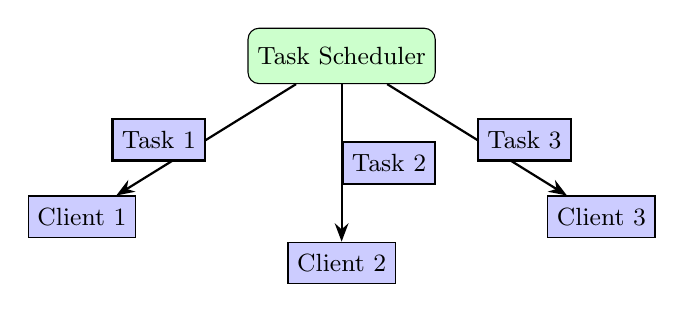
\begin{tikzpicture}[
    node distance=2cm,
    every node/.style={draw, fill=blue!20, text centered, minimum height=1.5em, font=\small},
    arrow/.style={-Stealth, thick},
    component/.style={draw, fill=green!20, rounded corners, text centered, minimum height=2em, font=\small}
    ]
    \node (scheduler) [component] {Task Scheduler};
    \node (client1) [below left=of scheduler] {Client 1};
    \node (client2) [below=of scheduler] {Client 2};
    \node (client3) [below right=of scheduler] {Client 3};
    
    \draw[arrow] (scheduler) -- (client1) node[midway, left] {Task 1};
    \draw[arrow] (scheduler) -- (client2) node[midway, right] {Task 2};
    \draw[arrow] (scheduler) -- (client3) node[midway, right] {Task 3};
\end{tikzpicture}
\centering\caption{System Architecture: Task Scheduler and Clients}
\end{figure}

\begin{itemize}
    \item \textbf{Client to Scheduler:} Clients send status updates to the scheduler and request new tasks upon completion.
    \item \textbf{Scheduler to Client:} The scheduler assigns tasks to clients and receives completion acknowledgments.
\end{itemize}

\section{Practical Implementation}
\label{sec:section5}
\subsection{System Architecture Implementation}
The system implementation closely follows the theoretical architecture, though some limitations were encountered. Docker was used to simulate the distributed environment, with each client running in a separate container. The scheduler, built in Python, utilizes Flask to establish a RESTful API connection for communication between components. For a detailed view of the code and project structure, the files are available on GitHub at: \url{https://github.com/danyagomezcantu/Verteilte_Systeme_Projekte}.

\subsection{Code Documentation}

The project consists of three key modules: \textit{client}, \textit{scheduler} and \textit{testing}, each responsible for a different aspect of the system. Below is a detailed breakdown of the main components and their functionalities.

% UML
\begin{figure}[h!]
\centering
\resizebox{\textwidth}{!}{
\begin{tikzpicture}[show background grid]
    % Package representing the entire project
    \begin{package}{system}
    
        % Client Module
        \begin{class}{Client}{-12,5}
            \attribute{api : API}
            \attribute{tasks : [ ]}
            \attribute{status : String}
            
            \operation{get\_status() : String}
            \operation{terminate()}
            \operation{run()}
        \end{class}
        
        \begin{class}{API}{-4.4,4.8}
            \attribute{app : Flask}
            \attribute{client : Client}
            
            \operation{create\_task\_from\_data(data) : Task}
            \operation{setup\_routes()}
        \end{class}
        
        % Scheduler Module
        \begin{interface}{Scheduler Interface}{-8,0}
            \attribute{tasks : List[Task]}
            
            \operation{add\_task(task : Task)}
            \operation{run()}
            \operation{\_sort()}
        \end{interface}
        
        \begin{class}{Scheduler}{-1,0}
            \inherit{Scheduler Interface}
            \attribute{waiting\_queue : List[Task]}
            
            \operation{execute()}
            \operation{assign\_task(client, task)}
            \operation{terminate\_clients()}
        \end{class}
        
        % Task Module
        \begin{class}{Task}{-8,-5}
            \attribute{name : String}
            \attribute{dataset : Dataset}
            
            \operation{execute()}
            \operation{task\_to\_json() : JSON}
        \end{class}
        
        % Testing Module
        \begin{class}{API Testing}{-12,-9}
            \operation{create\_client(dock) : Client}
            \operation{\_get\_host\_port(id) : String}
            \operation{\_get\_client\_ip(id) : String}
        \end{class}
        
        % Associations and Implementations
        \implements{Scheduler}{Scheduler Interface}
        \aggregation{Scheduler Interface}{tasks}{*}{Task}
        \association{Client}{API}
        \association{API}{Client}
        \association{API Testing}{Client}
    \end{package}
\end{tikzpicture}
}
\caption{UML Diagram of API Integration within the Task Scheduling System}
\end{figure}

\subsubsection{Client Module}

The Client Module is responsible for handling tasks and managing client-side operations, including interaction with the task scheduler and API. The module also includes the deployment configuration using Docker to ensure consistent and isolated environments for the application. Below is a detailed breakdown of the key components within this module.

\begin{itemize}{
    \item \textbf{REST\_API.py}
    \begin{itemize}
        \item \textbf{Libraries:}
        \begin{itemize}
            \item \texttt{from flask import Flask, jsonify, request}
        \end{itemize}
        \item \textbf{Methods:}
        \begin{itemize}
            \item \textbf{\_\_init\_\_(self, client)}: Initializes the API object with a reference to the \texttt{client} and sets up the Flask app.
            \item \textbf{create\_task\_from\_data(self, data)}: A placeholder method intended to convert received JSON data into a task object. Needs implementation.
            \item \textbf{setup\_routes(self)}: Sets up the API routes for checking status, terminating the client, and adding tasks.
            \item \textbf{status()}: Returns the status of the client in JSON format.
            \item \textbf{terminate()}: Terminates the client and returns a JSON response confirming the termination.
            \item \textbf{add\_task()}: Receives task data via POST, converts it into a task object, and adds it to the client's task queue.
            \item \textbf{run(self)}: Runs the Flask app on a specified host and port, enabling the API to listen for incoming requests.
        \end{itemize}
    \end{itemize}

    \item \textbf{client.py}
    \begin{itemize}
        \item \textbf{Libraries:}
        \begin{itemize}
            \item \texttt{import queue}
            \item \texttt{from enum import Enum}
            \item \texttt{import threading}
            \item \texttt{from REST\_API import API}
        \end{itemize}
        \item \textbf{Methods:}
        \begin{itemize}
            \item \textbf{\_\_init\_\_(self)}: Initializes the client, setting up the communication interface, status, task queue, and termination flag.
            \item \textbf{add\_task(self, task)}: Adds a task to the client's task queue.
            \item \textbf{\_isconnected(self)}: Checks if the client is connected to the network or server.
            \item \textbf{\_tasks\_available(self)}: Checks if there are tasks available in the queue to process.
            \item \textbf{terminate(self)}: Terminates the client by setting the termination flag.
            \item \textbf{get\_status(self)}: Returns the current status of the client (e.g., "working" or "waiting").
            \item \textbf{start(self)}: Starts the client's main loop, processing tasks from the queue and handling communication.
        \end{itemize}
    \end{itemize}

    \item \textbf{Dockerfile}
    \begin{itemize}
        \item The \texttt{Dockerfile} defines the environment setup for the client application, specifying how the Docker image should be built and what dependencies are needed. It ensures that the application can run consistently across different environments.
        \item \textbf{Instructions Included:}
        \begin{itemize}
            \item \textbf{FROM:} Specifies the base image (e.g., Python 3.10.11) to be used.
            \item \textbf{WORKDIR:} Sets the working directory inside the container to \texttt{/app}.
            \item \textbf{COPY:} Copies the necessary files, including the client, REST API, and requirements file, into the working directory.
            \item \textbf{RUN:} Executes commands to install Python dependencies required by the client.
            \item \textbf{EXPOSE:} Exposes the container's port (e.g., 5000) to the host machine.
        \end{itemize}
    \end{itemize}

    \item \textbf{requirements.txt}
    \begin{itemize}
        \item The \texttt{requirements.txt} file lists the Python dependencies required by the client application, ensuring that all necessary packages are installed within the Docker container.
        \item \textbf{Dependencies:}
        \begin{itemize}
            \item \texttt{Flask==3.0.3}
            \item \texttt{requests==2.32.3}
        \end{itemize}
    \end{itemize}
\end{itemize}

\subsubsection{Scheduler Module}
    \begin{itemize}
        \item \textbf{main.py}
        \begin{itemize}
            \item \textbf{Libraries:}
            \begin{itemize}
                \item \texttt{import numpy as np}
                \item \texttt{import pandas as pd}
                \item \texttt{from task import *}
                \item \texttt{from scheduler import *}
            \end{itemize}
            \item \textbf{Methods:}
            \begin{itemize}
                \item \textbf{\_\_init\_\_(self, dataset, time\_complexity=None)}: Initializes the main scheduler with a dataset and optionally a time complexity.
                \item \textbf{\_taketime(self)}: Measures and returns the time taken to execute the sorting task.
                \item \textbf{\_start(self)}: Marks the start time of the sorting operation.
                \item \textbf{\_end(self)}: Marks the end time of the sorting operation.
                \item \textbf{\_sort(self)}: Placeholder method for the sorting algorithm; expected to be overridden by subclasses.
                \item \textbf{get\_time\_complexity(self)}: Returns the time complexity of the sorting algorithm.
                \item \textbf{sort(self)}: Executes the full sorting process, including start, sorting, end, and time measurement.
            \end{itemize}
        \end{itemize}

        \item \textbf{scheduler.py}
        \begin{itemize}
            \item \textbf{Libraries:}
            \begin{itemize}
                \item \texttt{import task}
            \end{itemize}
            \item \textbf{Methods:}
            \begin{itemize}
                \item \textbf{add\_task(self, task)}: Adds a task to the scheduler's queue.
                \item \textbf{run(self)}: Runs the scheduler, processing tasks from the queue.
                \item \textbf{\_sort(self)}: Defines the sorting algorithm for the tasks in the scheduler. This method needs to be implemented by specific sorting algorithms.
            \end{itemize}
        \end{itemize}

        \item \textbf{task.py}
        \begin{itemize}
            \item \textbf{Methods:}
            \begin{itemize}
                \item \textbf{\_\_init\_\_(self, dataset, time\_complexity)}: Initializes a task with a name and associated dataset.
                
                \item \textbf{task\_to\_json(self)}: Placeholder method, meant to convert the task's details into a JSON format for transmission via the API.
            \end{itemize}
        \end{itemize}
    \end{itemize}
\subsubsection{Testing Module}
    \begin{itemize}
        \item \textbf{API\_testing.py}
        \begin{itemize}
            \item \textbf{Libraries:}
            \begin{itemize}
                \item \texttt{import time}
                \item \texttt{from flask import Flask}
                \item \texttt{from src.client.REST\_API import API}
                \item \texttt{import docker}
                \item \texttt{import requests}
            \end{itemize}
            \item \textbf{Methods:}
            \begin{itemize}
                \item \textbf{create\_client(dock)}: Creates a new Docker container for the client and runs it. Handles exceptions if the container fails to start.
                \item \textbf{\_get\_host\_port(id)}: Retrieves the host port that is mapped to the container's internal port. Returns the host port if available, otherwise returns \texttt{None}.
                \item \textbf{\_get\_client\_ip(id)}: Constructs the client's IP address using the host port retrieved by \textbf{\_get\_host\_port()} and returns it for making requests to the client.
            \end{itemize}
        \end{itemize}
    \end{itemize}

\section{Development Process and Learning}
\subsection{Initial Implementation and Task Definition}
To achieve a proof-of-concept through prototyping, we began by defining the tasks and their associated sorting functionality. Next, we moved on to the design and implementation of the scheduler. For maintainability and future extensibility, we developed an abstract class to serve as the foundation for specific implementations of tasks and schedulers. Since the “First-Come, First-Served” (FCFS) scheduler is the simplest to implement, we started with that.

\subsection{Testing and Integration}
With the core components in place, we proceeded to the testing phase by writing a main script to integrate all elements. The main.py script is interactive, importing a pre-generated dataset of random numbers from a CSV file into an array. The user is prompted to select the tasks to perform, and each task receives the dataset as an argument during initialization. The user then selects the scheduling algorithm—currently, only the FCFS algorithm is implemented. The script creates two Docker containers, before initializing the scheduler, based on the predefined image “Vs\_client”, and saves their IDs for subsequent use by the scheduler. The scheduler is designed to manage all clients. We chose to test with only two clients to simplify the process and confirm the system’s multi-client capability without adding unnecessary complexity. Although the system is designed to accommodate more than two clients, this capability has not been thoroughly tested. As will be discussed in the following sections, everything up to the point of assigning tasks to the clients functioned as expected.

\subsection{Docker Configuration}
The next significant step in development was defining the Docker containers: determining what software should run within them, how they should handle external requests, and what kind of communication would be necessary. Up to this point, the work had been of moderate difficulty, but every task involving Docker presented substantial challenges, requiring extensive research and testing. We were not able to launch the Docker containers, as they lacked the necessary libraries to run properly. This is where the next software module, client.py, became essential.

\subsection{Client.py and API Implementation}
The client.py class is relatively straightforward. Its role is to run within the Docker containers and process all incoming tasks using the First-Come, First-Served principle. To accept tasks, it required some form of API. After researching available options, we discovered Flask, a well-established RESTful API framework for Python.
However, we encountered two significant issues during its implementation. First, we realized that Python objects cannot be directly sent via the API. Second, we needed to enable the client to listen for incoming requests while concurrently processing tasks. The first problem was quickly resolved by sending the dataset and the type of task to be performed via JSON, allowing the client to generate task instances internally. The second issue was addressed by introducing threads: the API runs in the main thread, while task processing occurs in a separate thread. The rationale for threading the task processing is that the API needs to remain available longer than the task processing thread. When a termination signal is received, the system can shut down the task thread before terminating the main API process. This approach seemed logical for ensuring orderly shutdowns, as it prioritizes the termination of dependent processes before the main process. Additionally, in the event of a thread failure, the API might still be available for debugging, assuming the appropriate features are implemented. To maintain a clean and organized code structure, we had to implement a separate API class. However, we were not yet able to fully resolve our REST API issues, which impeded testing from our side. Apart from that we were not able to fully asess the need for a "working/waiting" status, it's code is left in but might contain some logical errors.

\section{Results and Discussion}
Throughout our implementation process, we encountered several challenges that required problem-solving and adaptation. We wanted to implement the First-Come, First-Served scheduling strategy, as our intention was to test a straightforward approach to task management. Setting up the Docker environment proved particularly difficult due to our limited prior experience. While we were able to develop Python code to create containers, we cannot confidently claim full success in configuring and managing these containers, as we were unable to verify their functionality or access logs effectively.

\subsection{Challenges and Reflection}
The task of understanding and implementing different scheduling algorithms was more complex than anticipated. Although our initial goal was to implement and test multiple scheduling strategies, we only managed to implement the simplest one, FCFS. Unfortunately, we were unable to fully test even this basic implementation due to unresolved issues with the API and the lack of log visibility in the containers. The learning process was, therefore, more iterative than expected, involving frequent adjustments, but ultimately couldn't the system’s full functionality. \\

The comparison of different scheduling strategies (Table 1) illustrates the trade-offs between simplicity and performance. We infer that First-Come, First-Served would be easier to implement, but still inefficient compared to other strategies, particularly under heavy loads \cite{Tyagi & Gupta, 2018}. More sophisticated algorithms like Priority Scheduling and Round Robin are recommended for future implementation to enhance the system's responsiveness and fairness.

\section{Future Work and Recommendations}

Our intention with this project was to develop a functional task scheduler within a distributed system, utilizing Docker containers and various scheduling algorithms. While significant progress was made in laying the groundwork, several key objectives were not fully realized, and the system remains incomplete. The following areas were identified as critical for further development:

\begin{itemize}
\item \textbf{Implementation of Additional Scheduling Algorithms:} The project initially aimed to compare different scheduling algorithms, such as Shortest Remaining Time (SRT) and Multiple-Level Queues Scheduling. However, only the First-Come, First-Served (FCFS) algorithm was implemented. Future work should focus on integrating these additional algorithms and thoroughly testing their performance within the system.

\item \textbf{Completion of the Task Management API:}  REST\_API.py remains underdeveloped, with several key features missing. These include task management, error handling, and task monitoring capabilities. Completing the API should be a priority to ensure that the system can handle a wide range of task management scenarios effectively.

\item \textbf{Container Management and Monitoring:} While Docker containers were successfully created, their management and monitoring were not fully implemented. Future development should include the addition of logging and monitoring tools to track container performance and task execution. This would help in diagnosing issues and ensuring that the system runs as expected.
\end{itemize}

\subsection{Next Steps for a Functional Prototype}

To move the project from its current state towards a fully functional prototype, the following steps are recommended:

\begin{itemize}
\item \textbf{Refine and Test the Current Implementation:} Before adding new features, it is essential to refine the existing implementation. This includes debugging the current system, ensuring that the API functions correctly, and validating the FCFS scheduler. Thorough testing is needed to confirm that the basic system works as intended.

\item \textbf{Implement Error Handling and Logging:} One of the project's significant shortcomings was the lack of error handling and logging mechanisms. Adding these features will be crucial for debugging and ensuring that the system can handle unexpected scenarios without crashing.

\item \textbf{Conduct Performance Testing:} Once the system is stable, performance testing should be conducted. This includes stress testing the system under various loads to identify bottlenecks and optimize the system's performance. Testing different scheduling algorithms, once implemented, will also be necessary to compare their efficiency.
\end{itemize}

\subsection{Considerations for Future Development}

Looking beyond the immediate next steps, future development could explore several avenues:

\begin{itemize}
\item \textbf{Dynamic Scheduling Adjustments:} Future iterations could explore the possibility of dynamic adjustments to the scheduling algorithm based on real-time performance data. This would involve developing a feedback loop where the system adjusts its scheduling strategy based on the workload and system performance.

\item \textbf{Scalability and Deployment:} While the current project focused on a small-scale implementation, future work could involve scaling the system to handle more clients and tasks. This would require optimizing the Docker deployment and ensuring that the system remains stable as it scales.

\item \textbf{Integration with External Systems:} Another area for future exploration is the integration of the task scheduler with external systems, such as cloud-based services or other distributed systems. This would broaden the applicability of the project and allow it to be used in a wider range of environments.
\end{itemize}

\section{Conclusion}
This project provided a meaningful learning experience in task scheduling for distributed systems, an area we had limited prior knowledge in. Through self-guided research and experimentation, we improved our understanding of essential tools such as Docker containerization, RESTful API development using Flask, and task scheduling algorithms implemented in Python. Although the final system was not fully completed, we successfully implemented several foundational elements, including the First-Come, First-Served (FCFS) scheduler and a basic client-server setup using Docker.\\

The challenges we faced—particularly in configuring Docker containers and ensuring seamless API communication—proved to be more complex than initially expected. However, overcoming these obstacles significantly contributed to our understanding of distributed system design. Each iteration of the system allowed us to refine our approach and build a clearer picture of how to implement and improve task scheduling algorithms within a distributed environment.\\

While we did not meet all our original goals, this project marked substantial progress compared to our initial knowledge. The difficulties encountered served as valuable learning opportunities, highlighting the importance of debugging, incremental development, and thorough testing in software projects. These lessons will inform our future work and enhance our problem-solving skills in this field.\\

This project laid the groundwork for future work and experimentation with distributed systems. The experience, although challenging, provided us with practical insights and technical skills that will be essential in continuing to develop and refine the system in the future.

\section{References}

\begin{hangparas}{1cm}{1}
Docker Documentation. (n.d.). Overview of Docker. Retrieved on September 5th, 2024 from: \url{https://docs.docker.com/get-started/overview/}
\end{hangparas}

\vspace{0.5cm}

\begin{hangparas}{1cm}{1}
Docker Documentation. (n.d.). Dockerfile Reference. Retrieved on September 5th, 2024 from: \url{https://docs.docker.com/engine/reference/builder/}
\end{hangparas}

\vspace{0.5cm}

\begin{hangparas}{1cm}{1}
Jalali Khalil Abadi, Z., Mansouri, N. and Javidi, M.M. (2024). \textit{Deep reinforcement learning-based scheduling in distributed systems: a critical review. Knowledge and Information Systems.} Retrieved on August 29th, 2024 from: \url{https://doi.org/10.1007/s10115-024-02167-7}
\end{hangparas}

\vspace{0.5cm}

\begin{hangparas}{1cm}{1}
Karatza, H. (2004). \textit{Scheduling in Distributed Systems.} In: Calzarossa, M.C., Gelenbe, E. (eds) \textit{Performance Tools and Applications to Networked Systems.} MASCOTS 2003. Lecture Notes in Computer Science, vol 2965. Springer, Berlin, Heidelberg. Retrieved on August 29th, 2024 from: \url{https://doi.org/10.1007/978-3-540-24663-3_16}
\end{hangparas}

\vspace{0.5cm}

\begin{hangparas}{1cm}{1}
Merkel, D. (2014). Docker: Lightweight Linux Containers for Consistent Development and Deployment. \textit{Linux Journal, 2014}(239), 2. Retrieved on September 5th, 2024 from: \url{https://www.linuxjournal.com/content/docker-lightweight-linux-containers-consistent-development-and-deployment}
\end{hangparas}

\vspace{0.5cm}

\begin{hangparas}{1cm}{1}
Tyagi, R., Gupta, S.K. (2018). \textit{A Survey on Scheduling Algorithms for Parallel and Distributed Systems.} In: Mishra, A., Basu, A., Tyagi, V. (eds) \textit{Silicon Photonics and High Performance Computing. Advances in Intelligent Systems and Computing,} vol 718. Springer, Singapore. Retrieved on August 29th, 2024 from: \url{https://doi.org/10.1007/978-981-10-7656-5_7}
\end{hangparas}


\end{document}
